%!TEX root=../Thesis_Zepeng.tex
\chapter{Fatigue life calculation methods}\label{chp:2}
\minitoc

To obtain a better knowledge of the impact of different types of stresses and mechanism of energy dissipation in high cycle fatigue(HCF), many researchers have carried out tests often difficult to implement and to control. From the data obtained and sometimes from the observations of the associated mechanisms, they have developed models that account more or less faithfully for the experiment. The approaches used are quite varied, but since the field of fatigue that interests us (HCF) is often governed by crack initiation, we make the choice in this chapter to treat only models established in the framework of continuum mechanics. It will therefore be a question of the state of the art of the most successful existing models but above all we will try to compare the predictions obtained when dealing with the equivalent stress and energy dissipation. This study will make it possible to reveal the great variety of the predictions obtained and to direct our work towards a better understanding of the behavior for the loads appearing the most problematic.



\section{Basquin curve}

\vspace{6pt}
\textbf{Stress-Life Diagram (S-N Diagram)}
\vspace{6pt}

The basis of the Stress-Life method is the Wohler S-N diagram. The S-N diagram plots nominal stress amplitude S versus cycles to
failure N. There are numerous testing procedures to generate the required data for a proper
S-N diagram. S-N test data are usually displayed on a log-log plot, with the actual S-N line
representing the mean of the data from several tests.

\begin{figure}[h!]
	\centering
	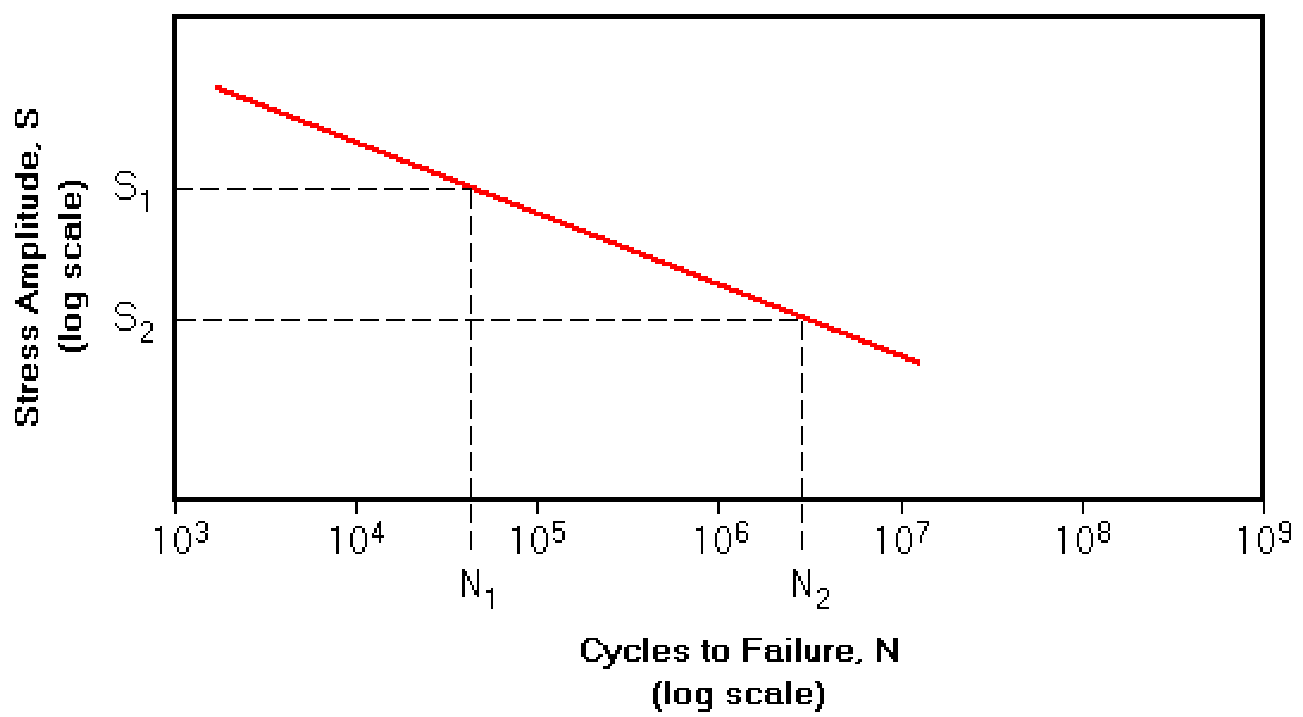
\includegraphics[width=0.8\textwidth]{figures//basquin.png} 
	\caption{Idealized S-N curve for high cycle fatigue.}
	\label{fig.basquin}
\end{figure}

Certain materials have a fatigue limit or endurance limit which represents a stress level below
which the material does not fail and can be cycled infinitely. If the applied stress level is below
the endurance limit of the material, the structure is said to have an infinite life. This is
characteristic of steel and titanium in benign environmental conditions. A typical S-N curve
corresponding to this type of material is shown in \figref{fig.basquin}.

Many non-ferrous metals and alloys, such as aluminum, magnesium, and copper alloys, do not
exhibit well-defined endurance limits. These materials instead display a continuously
decreasing S-N response. In such cases a fatigue strength $S_f$ for
a given number of cycles must be specified. An effective endurance limit for these materials is
sometimes defined as the stress that causes failure at $1\times10^8$ or $5\times10^8$ loading cycles.

The concept of an endurance limit is then used in infinite-life or safe stress designs. The possibility of infinite cycling is due to
interstitial elements (such as carbon or nitrogen in iron) that pin dislocations, thus preventing
the slip mechanism that leads to the formation of microcracks. Care must be taken when
using an endurance limit in design applications because infinite cycling potentiality can disappear due to:

\vspace{6pt}
$\bullet$ Periodic overloads (unpin dislocations)

$\bullet$ Corrosive environments (due to fatigue corrosion interaction)

$\bullet$ High temperatures (mobilize dislocations)
\vspace{6pt}     

The endurance limit by itself is not a true property of a material, since other significant influences such
as surface finish cannot be entirely eliminated. However, a test values ($S_e'$) obtained from
polished specimens provide a baseline to which other factors can be applied. Influences that
can then affect the endurance limit include:

\vspace{6pt}
$\bullet$ Surface Finish

$\bullet$ Temperature

$\bullet$ Stress Concentration

$\bullet$ Notch Sensitivity

$\bullet$ Size

$\bullet$ Environment

\vspace{6pt}         

\textbf{Power Relationship}   
\vspace{6pt}

When plotted on a log-log scale, an S-N curve can be approximated by a straight line as shown
in \figref{fig.basquin}. Basquin's equation is a power law relationship as  Eq.\eqref{eq.basquin} which describes the linear relationship between the applied stress cycles (S) in the y-axis and the number of cycles to failure in the x-axis plotted on a log-log scale.
\begin{equation}
N=BS^\frac{1}{b}
\label{eq.basquin}
\end{equation}
To calculate the slope of the Basquin equation from two significant curve points, we need to solve the system of equations:
$$N_1=N_2\left(\dfrac{S_1}{S_2}\right)^\frac{1}{b},$$
yielding
$$b=\dfrac{logS_1-logS_2}{logN_1-logN_2},$$
where $b$ is the slope of the line. Then the coefficient $B$ in Eq.\eqref{eq.basquin} is given by 
$$B=N_1S_1^{-\frac{1}{b}}=N_2S_2^{-\frac{1}{b}},$$
with $S_1$ denoting the stress range value of the considered test.

For the constant B, in industry  the stress range value (from the maximum cyclic stress to the minimum cyclic stress) is often considered. If the stress values of the S-N curve are given as alternating stresses (which is the common practice), multiply these stresses by 2 to calculate the constant B (stress range = 2* alternating stress, assuming a zero mean stress and full reversal of the cyclic load). If the S-N curve data are given in stress range values, apply them directly in the equation for estimating the constant B. 

The power relationship is only valid for fatigue lives that are on the design line. For ferrous metals this range is from $1\times10^3$ to $1\times10^6$ cycles. For non-ferrous metals, this range is from
$1\times10^3$ to $5\times10^8$ cycles. 

Basquin curves are quite simple but how can we apply them to more complex loadings?

\textit{This limitation is at the origin of the development of more detailed criteria to be described in the next section.}

\section{Basic fatigue criteria }
This bibliographic chapter reviews different methods to calculate the lifetime of multiaxial high cycle fatigue. In fact, the difficulty of defining the equivalent stress in situations with multiaxial loading and variable amplitude loading reveals the necessity of study these methods. These criteria allows to determine whether the stress trajectory in the stress space leads to the failure of the points concerned.

Papadopoulos suggested, in particular, to group families of fatigue criteria into four categories:
\begin{itemize}
	\item Criteria based on strain
	\item Criteria based on stress
	\item Criteria based on energy
	\item Criteria based on plasticity-damage coupling.
\end{itemize}
Generally, the criteria developed in strain and sometimes in energy are adapted to the oligocyclic fatigue where the tests are often carried out with imposed strain. Approaches in stress and sometimes in energy, as well as those based on the coupling of plasticity and damage which have begun to emerge in recent years are being applied in the domain of endurance. Therefore, we will focus on the last three categories and analyze the different approaches.

\subsection{Criteria based on stress}
\vspace{6pt}

Three types of approach can be distinguished:
\begin{itemize}
	\item Critical Plan Approaches
	\item Approaches based on stress invariants
	\item The criteria based on mean stress in an elementary volume
\end{itemize}
For simplicity and to avoid too costly identification procedures of fatigue data, criteria are often expressed using two
parameters to characterize the local load. The first relates generally to a shear stress (on a plane or on average over an elementary volume) while
the second reflects the normal stress effects (mean and amplitude) through the hydrostatic stress or the normal stress.
The criteria using the hydrostatic stress are the most numerous (\cite{crossland1956effect}, \cite{sines1959behavior}, \cite{FFE:FFE452}, \cite{thu2008effet}). The micro-macro approach applied to the field of endurance was born with the work of (\cite{van1973khmu}), and since it has been used many times, including by (\cite{papadopoulos1993fatigue}) to take better account of loading path effects.


Many fatigue limit criteria can thus be written as:
\begin{equation}
f(\tau)+g(\sigma) \leqslant 0
\label{eq.generalfatigue}
\end{equation}
where $f$ and $g$ are given functions of the shear stress $\tau$ and of the normal stress $\sigma$ respectively, as applied to different interfaces within the material.  

The normal and shear stress acting on the material planes and used in Eq.\eqref{eq.generalfatigue} are sometimes defined from a critical plane (\cite{findley1959behavior}), or
through integration at every plane of an elementary volume (\cite{liu1993berechnung}). \cite{thu2008effet} proposes, in
particular, a probabilistic approach based on this type of integration.

\vspace{6pt}
\textbf{Crossland Criterion}
\vspace{6pt}

 Using traditional fatigue criteria, a near hyperbolic relationship between stress and fatigue life is assumed, with an asymptotic limit defined as the endurance stress. To predict this asymptotic limit, the Crossland Criterion is probably the most widely known. Crossland proposed that the second invariant of the deviatoric stress tensor and the hydrostatic pressure are the variables governing the endurance limit. 

The classical Crossland criterion defines the fatigue limit of metallic specimens subjected to multi-axial in-phase cyclic stress (\cite{crossland1956effect}) : 
\begin{equation}f(\sqrt{J_{2,a}},P_{max})=\tau_{eq}+aP_{max}-b\leqslant 0\end{equation}

where $\tau_{eq}=\sqrt{J_{2,a}}$ measures  the amplitude of variation of the second invariant of the deviatoric stress  and $P_{max}$ is the maximum hydrostatic stress observed during a loading cycle. If $f(\sqrt{J_{2,a}},P_{max})$ is negative or null, there is no damage. If $f(\sqrt{J_{2,a}},P_{max})$ is positive, there is likely to be damage and hence limited endurance. The physical constants $a$ and $b$ are material constants that needs to be determined experimentally. The amplitude of the square root of the second invariant of the stress deviator can be defined, in general case, as the radius of the smallest hypersphere of the deviatoric stress path (\cite{Papadopoulos1997219}):
\begin{equation}\sqrt{J_{2,a}}=\frac{1}{\sqrt{2}}\min \limits_{\uline{\uline{S_1}}}\left\lbrace \max \limits_{t}\left( (\uline{\uline{S}}(t)-\uline{\uline{S_1}}):(\uline{\uline{S}}(t)-\uline{\uline{S_1}})\right)\right\rbrace .\end{equation}

Recall that the deviatoric stress $\uline{\uline{S}}$ associated to a stress tensor $\uline{\uline{\sigma}}$  is defined by
\begin{equation} \uline{\uline{S}}=\uline{\uline{\sigma}}-\frac{1}{3}\left( tr\uline{\uline{\sigma}}\right) \uline{\uline{\mathbbm{1}}}.
\end{equation}

The maximum value that the hydrostatic stress reaches during the loading cycle is on the other hand:
\begin{equation}
P_{max}=\max\limits_{t}\{\frac{1}{3}tr(\uline{\uline{\sigma(t)}})\}.
\end{equation}

For a proportional cyclic loading, if one introduces the two extreme stress tensors $\uline{\uline{\sigma^A}}$ and $\uline{\uline{\sigma^B}}$ observed during the loading path, together with the stress amplitude
\begin{equation}\uline{\uline{\Delta\sigma}}=\uline{\uline{\sigma^B}}-\uline{\uline{\sigma^A}}\end{equation}
and its deviatoric part $\uline{\uline{\Delta s}} $, the variation of
the second invariant of the stress deviator reduces to 
\begin{equation}
		\begin{split}
			\sqrt{J_{2,a}}&=\frac{1}{2\sqrt{2}}\max\limits_{t}\sqrt{\uline{\uline{\Delta s}}:\uline{\uline{\Delta s}}}\\&=\frac{1}{2\sqrt{2}}\max\limits_{t}\sqrt{(\Delta s_{11}^2+\Delta s_{22}^2+\Delta s_{33}^2+2\Delta s_{12}^2+2\Delta s_{13}^2+2\Delta s_{23}^2)}.
			\end{split}
	\end{equation}

The physical constants $a$ and $b$ can be related to  the limit $t_{-1}$ of endurance in alternate pure shear with $$P_{max}=0, \quad \uuline{\Delta s}=	\left(
\begin{array}{ccc}
0 & 2t & 0\\
2t & 0 & 0\\ 
0 & 0 & 0\\
\end{array}\right)  $$  
and to the limit $f_{-1}$ of endurance in alternate pure traction and compression where there is
$$P_{max}=\frac{1}{3}f, \quad \uuline{\Delta s}=	\left(
\begin{array}{ccc}
\frac{4}{3}f & 0 & 0\\
0 & -\frac{2}{3}f & 0\\ 
0 & 0 & -\frac{2}{3}f\\
\end{array}\right)  $$  
by
\begin{equation}
a=\frac{(t_{-1}-\frac{f_{-1}}{\sqrt{3}})}{\frac{f_{-1}}{3}}, \quad 
b=t_{-1}.
\label{eq.ab}
\end{equation}

Thus the classical Crossland criterion can be written as:
\begin{equation}
\sqrt{J_{2,a}}+a{P_{max}}-b\leqslant 0 .
\end{equation}
with $a$ and $b$ given by Eq.\eqref{eq.ab}.

\vspace{6pt}
\textbf{Dang Van Criterion}
\vspace{6pt}

In multiaxial fatigue with large number of cycles, the important role of local plasticity on the appearance of a fatigue limit is widely accepted and fully justifies the use of a multi-scale approach. Among the existing approaches, one of the most known and used is that of \cite{Van1999}. This criterion is used in particular in the design of certain automotive structures at PSA and
Renault. The criterion (\cite{van1986criterion}) belongs to the family of critical plane type approaches. The main physical
basis of this criterion focuses on the theory of elastic adaptation at two scales, mesoscopic and macroscopic. The macroscopic behavior of the material often remains elastic, only a grain oriented unfavorably undergoes
plastic deformation. The author states the following hypothesis: `` The
multiscale approach is settled on the assumption that under high cycle fatigue loading, a structure
will not be fractured by fatigue if an elastic shakedown is reached at the macroscopic scale as well
as at mesoscopic scale." (\cite{Van1999}). The approach developed first is
to describe the plasticity across the grain, assuming a yield criterion. The yield criterion is the law of Schmid with a
linear isotropic hardening. The author then search the elastic adaptation formula and defines a fatigue
test locally as shown in \figref{figDV} ($\Delta$ represents the tensor defining the orientation of the sliding system, $\gamma$ is the plastic slip  and $\tau$
is the amplitude of shear stress on the defined plan).
\begin{figure}[!h]
	\centering
	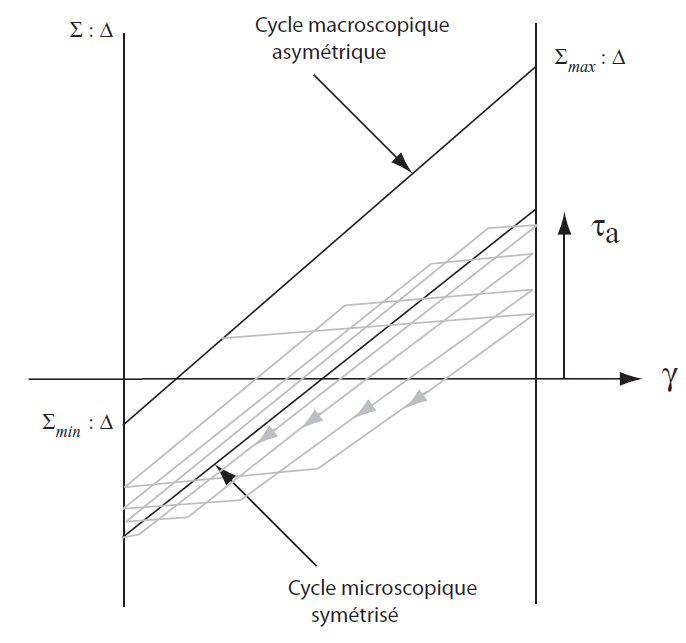
\includegraphics[width=0.7\textwidth]{figures//DV.png} 
	\caption{Elastic adaptation at the two scales (\cite{Van1999})}
	\label{figDV}
\end{figure}
Finally, a micro to macro upscaling strategy is applied to determine the criteria on the macroscopic scale. The localization law which is used is Lin-Taylor model that assumes equality of deformations at two scales. Using empirical relationships, the harmful role of the mean stress on the fatigue strength of the material is shown for type of uniaxial tensile stress. Dang Van shows the effect of the mean stress with  hydrostatic stress term in the criteria expressed as a linear combination of mesoscopic  shear stress on the maximum shear plane $\tau_a$ and the hydrostatic stress $\Sigma_H$.


The resulting Dang Van criterion presented in \cite{ballard1995high} is expressed as:
\begin{equation}
\max \limits_{\underline{n}}\left\lbrace \max \limits_{t}\left\{\tau_a{(\underline{n},t)}+a_D\Sigma_H(t)\right\}\right\rbrace \leqslant b_D.
\label{dv}
\end{equation}

where $\tau_a$ denotes the mesoscopic shear stress amplitude and is obtained from a mesoscopic stress tensor $\hat{\bm{\sigma}}$ defined by:
$$\hat{\uuline{\sigma}}(t)=(\uuline{\sigma}(t)-\uuline{s}^\star).$$
Here $\uuline{s}^\star$ is the center of the smallest hypersphere circumscribed to the loading path in deviatoric stress space. It is obtained by solving a ``min-max" problem as follows:
$$\uuline{s}^\star = arg \min\limits_{\underline{\underline{s}}_1}\left\{\max\limits_t\parallel \uuline{s}(t)-\underline{\underline{s}}_1\parallel\right\}.$$
In the case of fully reversed loading, the values $\uuline{s}^\star=0$ can be directly deduced without solving the ``min-max problem" as in general case.

The principal stress values of stress tensor $\uuline{\hat{\sigma}}$ being denoted by $\hat{\sigma}_{\Rmnum{3}}(t)\leqslant\hat{\sigma}_{\Rmnum{2}}(t)\leqslant\hat{\sigma}_{\Rmnum{1}}(t)$, one gets the amplitude of shear stress by:
$$\max \limits_{\underline{n}}\tau_a(t)=\frac{1}{2}(\hat{\sigma}_{\Rmnum{1}}(t)-\hat{\sigma}_{\Rmnum{3}}(t)).$$
Here $\Sigma_H(t)$is the hydrostatic stress as a function of the time, given by:$$\Sigma_H(t)=\frac{\sigma_{kk}(t)}{3}.$$
The Dang Van criterion then writes 
\begin{equation}
\frac{1}{2}\left( \hat{\sigma}_{\Rmnum{1}}(t)-\hat{\sigma}_{\Rmnum{3}}(t)\right) +a_D\dfrac{tr\left( \uline{\uline{\sigma}}\right) }{3}\leqslant b_D.
\end{equation}
The material characteristic parameters $a_D$ and $b_D$ of the Dang Van
criterion, can be related to the fully reversed bending or tension-
compression fatigue limit because of the same stress state between them, denoted by $f_{-1}$ (or $s_{-1}$), and to the torsion fatigue limit, denoted by $t_{-1}$,

$$a_D=\frac{3t_{-1}}{s_{-1}}-\frac{3}{2};$$  $$b_D=t_{-1}.$$

In the particular case of the uniaxial tension with average load $\Sigma_{xx,m}$ and amplitude $\Sigma_{xx,a}$, the criterion is written as:
$$\Sigma_{xx,a}\left(\dfrac{1}{2}+\dfrac{a_D}{3} \right)+\Sigma_{xx,m}\left(\dfrac{a_D}{3} \right) =b_D.$$

\vspace{6pt}
\textbf{Papadopoulos Criterion}
\vspace{6pt}

The approach proposed by \cite{papadopoulos1993fatigue} also uses the concept of elastic adaptation and even the localization law. According to him, ``the observations at the mesoscopic scale show that the initiation of a fatigue crack is
defined as the occurrence of micro-cracks corresponding to the rupture of the most deformed crystal grains in an
aggregate. Thus, a fatigue limit criterion can be modeled by a limit value of the accumulated plastic strain in the
most distorted grain."
$$\gamma_{cum}\leqslant\gamma_\infty.$$
He proposes to opt for a mean value of the accumulated plastic strain on all possible slip systems of representative elementary volume (REV). So he chose to use a average value  of accumulated plastic deformation rather than looking at failure of a single crystal. A spherical coordinate system is shown in \figref{fig50} to guide the normal vector in the material plane, and the unit direction vector $r$ linked to a sliding direction of this plan is used to conduct the integration over all possible orientations.

\begin{figure}[h!]
	\centering
	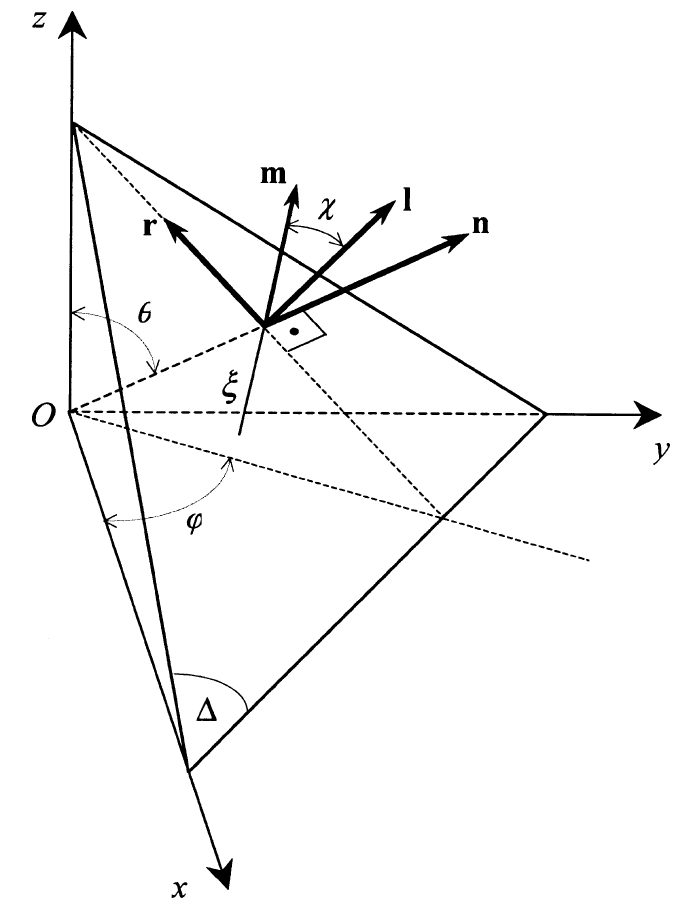
\includegraphics[width=0.5\textwidth]{figures//demopp.png} 
	\caption{Material plane $\Delta$ passing through point O of a body and its
		associated (n, l, r) frame(\cite{papadopoulos1993fatigue}).}
	\label{fig50}
\end{figure}
More precisely, at any point $O$ of a body, a material plane $\Delta$ can be defined by its unit normal vector $\bf n$. This vector
$\bf n$ makes an angle $\theta$ with the z-axis of a $Oxyz$ frame attached to the body, and its projection on the $xy$ plane
makes an angle $\varphi$ with axis $x$. For each plane $\Delta$ a new quantity is introduced called $generalised$ $shear$ $stress$ amplitude and denoted as $T_a$.This shear stress quantity was first introduced in \cite{papadopoulos2001long}
and was subsequently used by other researchers.The critical plane according to our proposal is that onto which $T_a(\varphi,\theta)$ achieves its maximum value. The fatigue limit criterion is written as:
\begin{equation}
max T_a+\alpha_\infty \Sigma_{h,max}\leqslant \gamma_\infty
\end{equation}
where $\alpha_\infty$ and $\gamma_\infty$ are material parameters to be determined (\cite{papadopoulos2001long}), and where we take
$$\Sigma_{h,max}=\max\limits_{t}\left\lbrace \frac{1}{3}tr(\uline{\uline{\sigma}}(t))\right\rbrace $$
To define $T_a$, he introduced the resolved shear stress $\tau$:
\begin{equation}
\begin{split}
\tau=&[sin\theta cos\varphi\sigma_{xx}+sin\theta sin\varphi\sigma_{xy}+cos\theta\sigma_{xz}](-sin\varphi cos\chi-cos\theta cos\varphi sin\chi)+\\&[sin\theta cos\varphi\sigma_{xy}+sin\theta sin\varphi\sigma_{yy}+cos\theta\sigma_{yz}](cos\varphi cos\chi-cos\theta sin\varphi sin\chi)+\\&[sin\theta cos\varphi\sigma_{xz}+sin\theta sin\varphi\sigma_{yz}+cos\theta\sigma_{zz}]sin\theta sin\chi .
\end{split} 
\label{eqres}
\end{equation}
It is clear that the resolved shear stress is a function of
$\varphi$, $\theta$, $\chi$ and of time $t$ in the case of variable loading, i.e. $\tau=\tau(\varphi, \theta, \chi, t)$. Upon fixing a couple $(\varphi, \theta)$ (i.e. a plane
$\Delta$) and an angle $\chi$ (i.e. a line $\xi$ on $\Delta$), one can define the amplitude of the resolved shear stress $\tau_a$, acting on $\Delta$
along $\xi$ by the formula:
\begin{equation}
\tau_a(\varphi,\theta,\chi)=\frac{1}{2}\big[\max \limits_{t\in P}\tau_a(\varphi,\theta,\chi ,t)-\min \limits_{t\in P}\tau_a(\varphi,\theta,\chi ,t)\big].
\end{equation}
Finally, for a given plane $\Delta$, i.e. for a fixed couple ($\varphi$, $\theta$),
the generalized shear stress amplitude $T_a$ is defined as:
\begin{equation}
T_a(\varphi,\theta)=\sqrt{\frac{1}{\pi}\int_{\chi=0}^{2\pi} \tau_a^2(\varphi,\theta,\chi)d\chi}
\label{Ta}
\end{equation}
We note the fatigue limit in fully reversed torsion $t_{-1}$ and the fatigue limit in fully reversed bending $f_{-1}$. From these two tests we get the parameters:
$$\gamma_\infty=t_{-1},$$ 
$$\alpha_\infty=3\left( \frac{t_{-1}}{f_{-1}}-\frac{1}{2}\right) .$$
The Papadopoulos fatigue limit criterion achieves the form (\cite{papadopoulos2001long}):
\begin{equation}
maxT_a+3\left( \frac{t_{-1}}{f_{-1}}-\frac{1}{2}\right) \Sigma_{h,max}\leqslant t_{-1}.
\label{eq:papadopoulos}
\end{equation}
In the particular case of the fully reversed uniaxial tension, the criterion is written as (\cite{papadopoulos2001long}):
$$\dfrac{\Sigma_{xx,a}}{2}+\alpha_\infty\dfrac{\Sigma_{xx,m}}{3} \leqslant\gamma_\infty$$
\textit{In conclusion of this part in stress based criteria, we need to observe that these criteria are all based on the notion of cyclic loading, which can be a limitation in general case.}
\subsection{Criteria based on energy}
Depending on the type of density of deformation energy considered per cycle, the
Energy criteria are divided into three groups (\cite{macha1999energy}):
\begin{itemize}
	\item  criteria based on elastic energy
	\item  criteria based on plastic energy
	\item  criteria based on the sum of elastic and plastic energies.
\end{itemize}

The criteria based on the elastic deformation energy can be used in fatigue with a large number of cycles, whereas those based on the plastic deformation energy are more suitable for oligocyclic fatigue.

\cite{ellyin1974criterion} is one of the first to propose a fatigue criterion based on cyclic shear deformation energy. This approach was taken up and complemented by \cite{lefebvre1981cognitive} and \cite{ellyin1991phase} for the case of multiaxial loadings. In France, this approach is reflected in the work of \cite{Froustey1992} and then in \cite{palin1996fatigue} and \cite{banvillet2001prevision}.

\subsubsection{Energy dissipation based on strain energy density}

In their fatigue criterion, \cite{Froustey1992}  have considered a complete cycle of
stresses. They use the mean value on one cycle of
the volumic density of the elastic strain energy, $W_a$, whatever the point
M in the mechanical part.

$$W_a(M)=\frac{1}{T}\int_{0}^{T}\frac{1}{2}\sigma_{ij}(M,t)\varepsilon_{ij}^e(M,t)dt$$

where $\sigma_{ij}(M,t)$ and $\varepsilon_{ij}^e(M,t)$ are respectively the tensor of stresses and the tensor of
elastic strains at the considered point $M$ function of time $t$.  Thus, in low cycle fatigue $W_a$ can be considered as the mean value on one
cycle of the total strain energy density at the considered point. However, in high cycle fatigue usually the endurance limit
is low enough to consider that the material remains elastic at the macroscopic scale (\cite{chaboche1988non}).

In 1998 Thierry PALIN-LUC and Serge LASSERRE (\cite{palin1998energy}) proposed a failure criterion based on $W_a$. Their studies show that another limit, called $\sigma^*$, can be defined below
the usual endurance limit of the material, $\sigma_D$. At a considered point a stress amplitude
below this new limit does not initiate observable damage at the microscopic scale (no
micro-cracks). Two static characteristics of the material are necessary: $E$ and $\nu$. Three
experimental endurance limits under fully reversed loadings are needed: the endurance
limit in traction,$\sigma_{Trac,-1}^D$, the endurance limit in rotative bending, $\sigma_{RotBend,-1}^D$, and the
endurance limit in torsion, $\tau_{To,-1}^D$. 

This stress limit $\sigma^*$ can be estimated from
fatigue test results in fully reversed tension and in rotating
bending

$$\sigma^*=\sqrt{2(\sigma_{Trac,-1}^D)^2-(\sigma_{RotBend,-1}^D)^2}.$$

From $\sigma^*$ and by analogy with a sinusoidal traction load the corresponding mean value
of the strain energy volumetric density, $W_{a^*}$, can be calculated , where E is the
Young modulus of the material.

$$W_{a^*}=\frac{\sigma^{*2}}{4E}.$$

Around each point it is always possible to define
the volume $V^* (C_i)$ by the set of points M where $W_a (M)$ is higher than $W_{a^*} (C_i)$
. They postulate that the part of $W_a (M)$ exceeding $W_{a^*} (C_i)$ is the damaging part
of the strain energy volumetric density. They thus calculate $\overline{\omega}_a(C_i)$ 
the volumetric mean value of the strain energy around the critical point $C_i$

$$V^*(C_i)=\lbrace points\; M(x,y,z) \;around\; C_i \;such\; that \;W_a(M)\geqslant W_{a^*}(C_i) \rbrace$$

$$\overline{\omega}_a(C_i)=\frac{1}{V^*(C_i)}\int\int\int_{V^*(C_i)}^{}[W_a(x,y,z)-W_{a^*}(C_i)]d\nu$$

At the endurance limit and at the critical point $C_i$, this new quantity $\overline{\omega}_a(C_i)$ is
supposed to be constant, whatever the uniaxial stress state. If we note $\overline{\omega}_a^D(Uniax)$ its
value at the endurance limit for any uniaxial stress state our criterion can be written by
Eq.\eqref{eq.palinfailure}. Failure occurs if this equation is not verified.
\begin{equation}
\overline{\omega}_a(C_i)\leqslant\overline{\omega}_a^D(Uniax).
\label{eq.palinfailure}
\end{equation}

\textit{The limitation of this criterion is that it only deals with constant amplitude load case.}

\subsubsection{A critical plane approach based on energy concepts}


\cite{lagoda1999critical} proposed that under multiaxial loadings the normal strain energy density in the critical plane (i.e. the plane of the maximum damage) to be the energy parameter and translated into deformation or stress amplitude in a given experimental fatigue curve. The history of strain energy density is schematized with use of the rain-flow algorithm. %(\cite{\label{sec:5.1}})
Fatigue damage is accumulated according to Palmgren-Miner hypothesis and endurance limit uses the standard fatigue characteristic of the material, rescaled with use of the considered energy parameter. 
\begin{equation}W(t)=\frac{1}{2}\sigma(t)\varepsilon(t)sgn[\sigma(t),\varepsilon(t)]\label{eq.lagodaWt}
\end{equation}
$$sgn(x,y)=\frac{sgn(x)+sgn(y)}{2}$$

$sgn(x),sgn(y)=0,1,-1$ for distinguishing positive and negative works in a
fatigue cycle. Thus, it allows
to distinguish energy (specific work) for tension and
energy (specific work) for compression. 

If the stress and strain reach their maximum values,
$\sigma_a$ and $\varepsilon_a$, then the maximum energy density value is
\begin{equation}
W_a=\frac{1}{2}\sigma_a\varepsilon_a
\label{eq.lagodaWa}
\end{equation}

Taking $W(t)$ as the fatigue damage parameter according to Eq.\eqref{eq.lagodaWt}, we can rescale the standard characteristics of cyclic fatigue ($\sigma_a-N_F$) and ($\varepsilon_a-N_F$) and obtain a new one, ($W_a-N_F$ ). In the case of high-cycle fatigue, when the characteristic curve ($\sigma_a-N_F$) is used in order to predict the number of cycles $N_F$ to failure, the axis $\sigma_a$ should be replaced by $W_a$, where $W_a$ and $\sigma_a$ are related by:

$$W_a=\frac{\sigma_a^2}{2E}.$$

In the case of low and high-cycle fatigue, when the
characteristic ($\varepsilon_a-N_F$) is used, we can do similar rescaling. 
%We assume $$\sigma_a=\sigma_f'(2N_F)^b$$
%
%From Manson-Coffin-Basquin equation  and Eq.\eqref{eq.lagodaWa} we obtain
%
%$$\varepsilon_a=\varepsilon_a^e+\varepsilon_a^p=\frac{\sigma_f'}{E}(2N_F)^b+\varepsilon_f'(2N_F)^c$$
%$$W_a=\frac{1}{2}\sigma_a\varepsilon_a=\frac{\sigma_a}{2}\left[\frac{\sigma_f'}{E}(2N_F)^b+\varepsilon_f'(2N_F)^c\right]=\frac{(\sigma_f')^2}{2E}(2N_F)^{2b}+0.5\varepsilon_f'\sigma_f'(2N_F)^{b+c}$$
%
%Fatigue characteristic for high-cycle fatigue
%takes the form
%$$W_a=\frac{(\sigma_f')^2}{2E}(2N_F)^{2b}$$

The full approach is described in \figref{fig.algorithm}. Having tensors of strain and stress histories we can
determine histories of normal strain energy density (stage
3) in all the planes according to Eq.\eqref{eq.lagodaWt} with the distinguished direction $\bar{\eta}$.
\begin{equation}
W_{\eta}(t)=0.25\varepsilon_\eta(t)\sigma_\eta(t)[sgn\varepsilon_\eta(t)+sgn\sigma_\eta(t)]
\label{eq.lagodaWeta}
\end{equation}
where
\begin{equation}
\sigma_\eta(t)=[\hat{l}^2_\eta\sigma_{xx}(t)+\hat{m}^2_\eta\sigma_{yy}(t)],
\label{eq.lagodasigeta}
\end{equation}
\begin{equation}\varepsilon_\eta(t)=[\hat{l}^2_\eta\varepsilon_{xx}(t)+\hat{m}^2_\eta\varepsilon_{yy}(t)+\hat{n}^2_\eta\varepsilon_{zz}(t)],\label{eq.lagodavareta}
\end{equation}
with $\hat{l}^2$, $\hat{m}^2$, $\hat{n}^2$ = direction cosines of the unit vector $\bar{\eta}$.

In the plane stress state, the normal vector orientation
to the fracture plane may be described with use of one
angle $\alpha$ in relation with the x-axis. Thus, the direction
cosines of the axis $\bar{\eta}$ are:
$\hat{l}_\eta=cos\alpha$, $\hat{m}_\eta=sin\alpha$, $\hat{n}_\eta=0$.
\begin{figure}[h!]
	\centering
	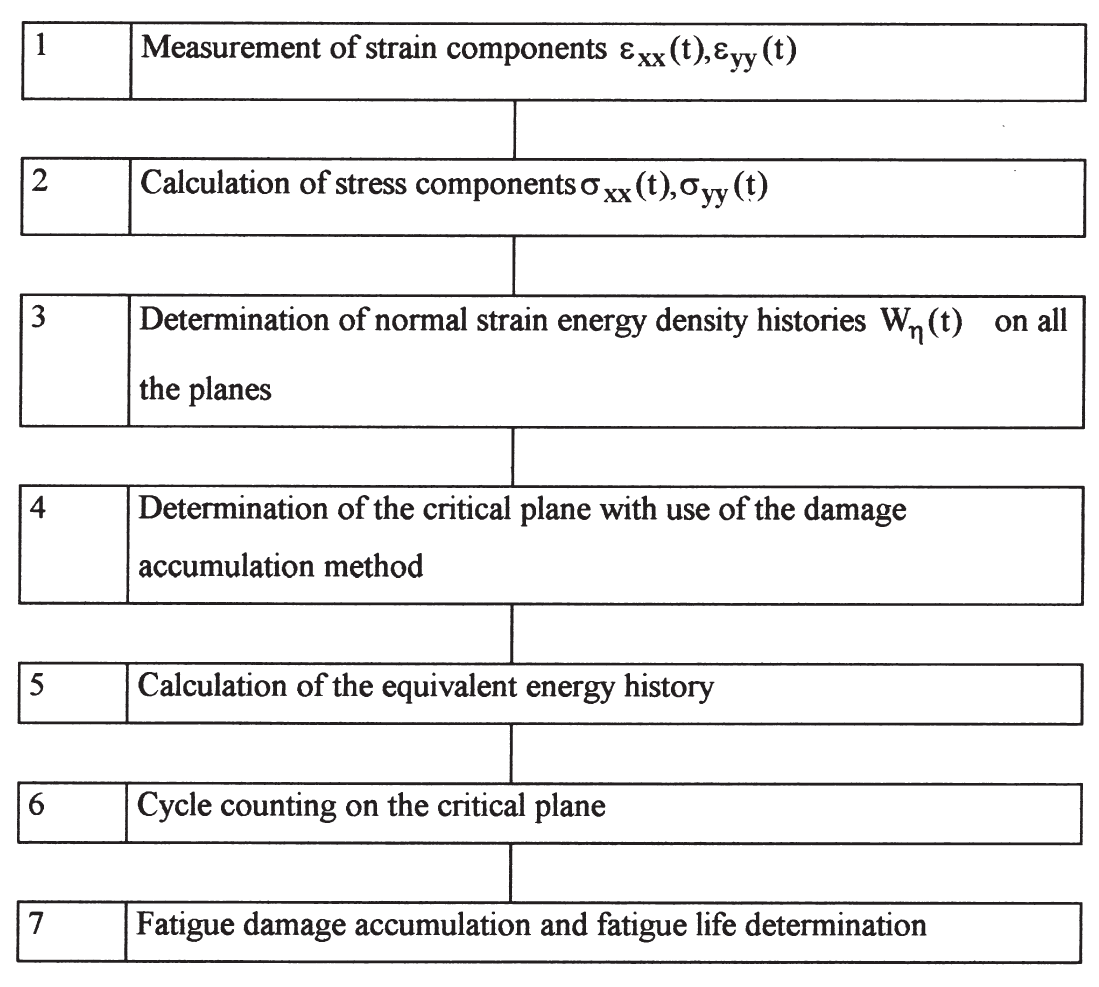
\includegraphics[width=0.7\textwidth]{figures//algorithm.png} 
	\caption{Algorithm of fatigue life determination with use of the energy parameter in the critical plane under biaxial random tension-compression (\cite{lagoda1999critical}).}
	\label{fig.algorithm}
\end{figure}
In stage 4 the critical plane is determined by choosing the plane of maximal energy variation $\max \limits_{\eta}\Delta W_{\eta}(t)$ according to
the damage accumulation method Eq.\eqref{eq.lagodaWeta}. Fatigue lives
were determined at particular expected planes according
to the following stages. When the energy density history
at the given plane in stage 6 has been determined, the
energy cycles are counted with the rain flow method;
next damage is accumulated according to Palmgren-
Miner hypothesis taking into account energy
cycles of amplitude larger than a $W_{af}$ (with $a=\frac{1}{4}$ and $W_{af}$ the fatigue limit expressed in strain energy density).
$$S(T_0)=\sum_{i=1}^{j}\dfrac{n_i}{N_0(W_{af}/W_{ai})^{m'}} \qquad for \quad W_{ai} \geqslant aW_{af},$$
$$S(T_0)=0 \qquad for \quad W_{ai} \leqslant aW_{af},$$
where $S(T_0)$ is material damage up to time $T_0$ ; $j$ is number of class intervals of the histogram of the amplitudes
of the strain energy density; $W_{af}$ is fatigue limit
expressed by strain energy density;  $m'$ is slope of fatigue curve; $N_0$ is a number of cycles corresponding to the fatigue
limit $W_{af}$ ; $n_i$ is a number of cycles with amplitude $W_{ai}$.

When the degree of damage at observation time $T_0$ is
determined, the fatigue life is calculated by extrapolation:
$$T_{cal}=\dfrac{T_0}{S(T_0)}.$$

\textit{This method is able to handle general loadings, but still requires cycle counting. And the determination of critical plane in multiaxial load is laborious. Also, they use the Miner's damage law which can not account for the sequencing effect.}

\subsubsection{Lamefip Criterion}
The so-called Lamefip criterion, presented here with its latest version (\cite{benabes2006approche}), makes it possible to handle all types of loads and to take into account the effect of the stress gradients. This criterion is based on the notion of the volume of influence around the ``critical point" and uses as a parameter the volume density of straining work supplied per cycle to each volume element.

\cite{ellyin2012fatigue} showed that the use of both the plastic and elastic strain work can be used
as damage parameter in multiaxial fatigue. The LAMEFIP criterion (\cite{banvillet2003volumetric}),
devoted to the field of endurance or limited endurance, uses for damage parameter, the volumetric density of the strain work given to the material per loading cycles after elastic shakedown is supposed to be reached after a few thousands cycles.

The proposal is based on two main hypothesis : (i) the strain work given to the material per loading cycle is considered as the driving force for fatigue crack initiation and (ii) it is calculated after macroscopic elastic shakedown.

Many authors use cycle counting techniques (chapter \ref{chp:4}) to extract, from a random stress tensor sequence, cycles from which the damage could be estimated. These techniques have two main drawbacks : (i) the choice of the cycle counting algorithm influences the calculated fatigue life since the number of counted cycles is algorithm dependent (\cite{dowling1983fatigue}), and (ii) for multiaxial non-proportional stress states, in many approaches from the literature, the variable chosen for cycle counting differs from the damage parameter. To avoid such drawbacks an incremental model has been developed. The strain work density given at a point M is written in an incremental way as follows :

$$dW_g(M,t)=\sum_{i=1}^{3}\sum_{j=1}^{3}\left\langle \sigma_{ij}\left( M,t\right)\dot{\epsilon}_{ij}\left( M,t \right)\right\rangle  dt .$$

\noindent
- where $\epsilon_{ij}\left( M,t\right)$ are the strain tensor components and $\dot{x}= dx/dt$,\\
- $\sigma_{ij}\left( M,t\right)$ are the stress tensor components,\\
- and $\left\langle m\right\rangle$ gives the positive value of $m$ according to : $\left\langle m\right\rangle=1$ if $m \geqslant 0$; $\left\langle m\right\rangle=0$  if $m < 0$.

As underlined by \cite{ellyin2012fatigue}, the strain work can be calculated as the sum of elastic and plastic strain works, so that :
$$dW_g(M,t)=dW_g^e(M,t)+dW_g^p(M,t).$$
The framework of this study being HCF and MCF, they choose to consider only the elastic part of the strain work (Eq.\eqref{eq.lamefip1}) in the elastic shakedown state. The cumulated strain work on a time
sequence of duration $T$ is equivalent to the integral of $dW_g^e(M,t)$ over $T$ as in Eq.\eqref{eq.lamefip2}. \cite{banvillet2003volumetric} has shown that for an uniaxial stress state $W_g$ is not shape dependent (sinus, triangle,square, etc...).
\begin{equation}
dW_g^e(M,t)=\sum_{i=1}^{3}\sum_{j=1}^{3}\left\langle\sigma_{ij}\left( M,t\right)\dot{\epsilon}_{ij}^e\left( M,t\right)\right\rangle dt .
\label{eq.lamefip1}
\end{equation}
\begin{equation}W_g(M,T)=\int_{t}dW_g(M,t).\label{eq.lamefip2}
\end{equation}

To take into account the material sensitivity to the stress triaxiality, the triaxiality degree, $dT$, at a point M is defined by the ratio of the strain work associated with the spherical part of the stress tensor over the total strain work of \cite{banvillet2003volumetric}, but in an incremental way :
$$dT(M,t)=\dfrac{dW_g^{Sph}(M,t)}{dW_g(M,t)} \qquad if \qquad  dW_g(M,t)\neq0,\ otherwise \quad dT(M,t)=0,$$
with
$$dW_g^{Sph}(M,t)=\left\langle \dfrac{1}{3}\sum_{k=1}^{3}\sigma_{kk}(M,t)\sum_{l=1}^{3}\dot{\epsilon}_{ll}^e(M,t)\right\rangle dt.$$
The material sensitivity to stress triaxiality is considered by using an empirical function
$F(dT,\beta_m)$ (Eq.\eqref{eq.lamefip3}) depending on the material parameter $\beta_m$ identified from two fully reversed
fatigue limits (rotating bending and torsion). At any instant, for a multiaxial stress state, the
strain work given to the material is corrected to evaluate an uniaxial equivalent strain work
$d{W_f}_{eq} (M,t)$ (Eq.\eqref{eq.lamefip4}):
\begin{equation}
F(dT(M,t),\beta_m)=\dfrac{1}{1-dT(M,t)}\left[ 1-\dfrac{1}{\beta_m}ln\left[1+dT(M,t)(e^{\beta_m}-1) \right] \right] .
\label{eq.lamefip3}
\end{equation}
\begin{equation}
d{W_g}_{eq} (M,t)=d{W_g}(M,t)\dfrac{F(dT_{uniax},\beta_m)}{F(dT(M,t),\beta_m)}.
\label{eq.lamefip4}
\end{equation}
A threshold $W_g^*$ is introduced. It represents the volume density of the minimum elastic deformation work to be provided to create, after a large number of cycles, irreversible damage in a REV. The volume influencing fatigue crack initiation $V^*$ is thus
defined whatever the stress state is at the critical point.
\begin{equation}
W_g^*=W^*_{g,uniax}\dfrac{F(dT_{C_i},\beta_m)}{F(dT(uniax),\beta_m)}.
\label{eq.lamefip5}
\end{equation}
\begin{equation}
V^*(C_i)=\left\lbrace points \; M(x,y,z) \; around \; C_i \; so \; that \; {W_g}_{eq} (M,t)\geqslant W_g^*\right\rbrace .
\label{eq.lamefip6}
\end{equation}

 Assuming that the set of points of the volume of influence plays a significant role in the initiation of a fatigue crack at the critical point $C_i$, the volume mean value of the damaging work provided in the $V^*$ of influence is written:

$${W_g}_{C_i}=\dfrac{1}{V^*(C_i)}\int_{V^*(C_i)}\left[{W_g}_{eq}(M,T)- W_g^*\right] $$

In the case of uniaxial loading, the values of $W_g^*$ which serves as reference in Eq.\eqref{eq.lamefip5} are given by:
$$W^*_{g,uniax}=\dfrac{2s_{-1}^2-f_{rot-1}^2}{E}$$
$f_{rot-1}$ and $s_{-1}$ denote respectively the endurance limits in alternating rotational bending and traction.
The final criterion proposed by \cite{banvillet2003volumetric} is summarized in the following relation:
$${W_g}_{C_i}<{W_g}_{eq},$$

where ${W_g}_{eq}$ is the permissible limit value of ${W_g}_{C_i}$  at the limit of fatigue.

\textit{This approach is possible to predict the $S–N$ curves from
	a uniaxial one since the proposal is load type and mean
	load sensitive. However, the threshold work is another form of the fatigue limit which can be inaccurate microscopically.}

\subsection{Criteria based on plasticity-damage coupling}
In recent years, a new class of criteria coupling mesoplasticity and damage has emerged.  \cite{lemaitre1999two} have, for example, used the approach introduced by \cite{lemaitre1985mecanique} based on the thermodynamics of irreversible processes and the mechanics of continuous media.  \cite{flaceliere2004contribution} also proposed a model based on a plasticity-damage coupling and attempted to account for the phenomena of damage observed experimentally on a C35 steel. In this work, we will focus on a more recent approach proposed by \cite{monchiet2006contributions}.
\subsubsection{Criterion of Monchiet et al}
In order to account for the coupling plasticity-damage in high cycle fatigue, \cite{monchiet2006contributions} uses a micro-mechanical approach based on the work of  \cite{gurson1977continuum}. The damage is represented by a magnitude $f$ related to the development of porosity in the sliding bands at the origin of the initiation of the fatigue cracks. 

The model  is built on the following main assumptions. 

\begin{itemize}
	\item  Initiation of cracks in sliding bands by the presence of a high level of porosity in these bands.
	\item A localization law gives access to the mechanical fields at the mesoscopic scale.
	\item The elastic adaptation concept is used to access local mechanical fields in a stabilized state.
	\item A plasticity potential of Gurson type is introduced on the mesoscopic scale in order to show the effects of the plasticity-damage coupling.
\end{itemize}

The function of charge used (with $\Delta$ tensor of order two defining the orientation of the system of slip considered and equals to 
$\dfrac{1}{2}\left(\underline{n}\otimes\underline{m}+\underline{m}\otimes\underline{n} \right)  $ where $\underline{n}$ is normal to slip plan and $\underline{m}$ the sliding direction)
\begin{equation}
F=\left( \dfrac{\overline{\overline{B}}:\overline{\overline{\Delta}}}{\tau_d}\right) ^2+2fcosh\left(\dfrac{\sqrt{3}}{2}\dfrac{B_h}{\tau_h}\right)-1-f^2\leqslant 0 ,
\label{eq.monchiet1}
\end{equation}
where $\overline{\overline{B}}=\overline{\overline{\Sigma}}-\overline{\overline{X}}$, with $\overline{\overline{\Sigma}}$ the macroscopic stress tensor and $\overline{\overline{X}}$ the  kinematic hardening variable. $\overline{\overline{X}}$  decomposes into a hydrostatic part $X_h$ and a slip component on the predominant system, denoted $X_d$. $\Sigma_H$. Isotropic hardening is introduced by replacing the plasticity threshold $\tau_0$ by two parameters $\tau_d$ and $\tau_h$.

Without going into the details of this model adapted to the problem of fatigue at large number of cycles, it seems very important, in order to understand the rest of the work, to resume the way in which hardening is introduced into the load function. The main difference with the conventional charge function proposed by Gurson is the existence of a isotropic combined kinematic hardening with decomposition into deviatoric parts (parameters $\tau_d$ and $X_d$) and hydrostatic (parameters $\tau_h$ and $X_h$).

To obtain the expressions of these variables, the authors follow the same approach as \cite{leblond1995improved}, by postulating paths of pure deviatoric stress and pure effect of fatigue damage at high mean hydrostatic values. The aim is to identify the parameters of hardening from specific exact solutions. The authors reach the relationships:
\begin{equation}\tau_d = \tau_0 + R_d
\label{eq.monchiet10}
\end{equation}
\begin{equation}\tau_h = \tau_0 + R_h
\label{eq.monchiet11}
\end{equation}
\begin{equation}R_d=R_0\gamma_{cum}
\label{eq.monchiet12}
\end{equation}
\begin{equation}R_h=hR_0\gamma_{cum}+R_0\xi_{cum}^h
\label{eq.monchiet13}
\end{equation}
with $R_0$ isotropic hardening parameter and $h$ latent hardening parameter. It is important to note that plastic slip $\gamma$ and the parameter $\xi^h$ are cumulative, due to applications to fatigue. In the rest of the presentation $\gamma_{cum}$ and $\xi_{cum}^h$
represent the quantities in the adapted state. For kinematic hardening, the parameters obtained are as follows:
\begin{equation}
X_d=((1-f)c)\gamma
\label{eq.monchiet14}
\end{equation}
\begin{equation}
X_h=\dfrac{2p_1c}{\sqrt{3}}\xi^h
\label{eq.monchiet15}
\end{equation}

with $c$ the parameter of kinematic hardening, $p_1$ the parameter of cubic anisotropy.
The variable $\xi^h$ equals :
\begin{equation}
\xi^h=\dfrac{2}{\sqrt{3}}\left\lbrace dilog\left(\dfrac{f_a}{f}\right) -dilog\left(1-f_g \right)  \right\rbrace 
\label{eq.monchiet16}
\end{equation}
with $dilog(x)=\int_{1}^{x}\dfrac{ln(x')}{1-x'}dx'$.

The criterion therefore postulates that a fatigue crack appears in a sliding band when the fraction of porosity inside this band reaches a critical value $f_c$

Plasticity occurs locally when the equivalent stress reaches the yield limit. The authors take into account two mechanisms of damage in the evolution of the porosity:

\vspace{6pt}
\begin{itemize}
	\item  The first is related to the creation of gaps by annihilation of dislocations. This mechanism is at the origin of the accumulation of point defects of the lacunar or interstitial type along the persistent slip bands (PSB). The phenomenological model proposed by \cite{essmann1979annihilation} gives access to the porosity $f_a$:
	\begin{equation}
	f_a= A_0\left\lbrace k_a\gamma_{cum}-1+exp\left(-k_a\gamma_{cum} \right)  \right\rbrace .
	\label{eq.monchiet2}
	\end{equation}
	
	\item  The second mechanism is related to the growth of micro-cavities. Using an incompressibility hypothesis, $f_g$ is defined by:
	\begin{equation}
	f_g=\left\lbrace 1-exp\left(3\epsilon_h^p \right) \right\rbrace.
	\label{eq.monchiet3}
	\end{equation}
\end{itemize}

It is important to note that the first mechanism involves the accumulated plasticity $\gamma_{cum}$, related to amplitude effects. The second mechanism depends on the hydrostatic plastic deformation $\epsilon_h^p$, and allows the taking into account of the mean stress effects.

The fatigue criterion is established on the basis of the following hypothesis: ``a sufficient condition for nucleation of a fatigue crack is obtained if the porosity reaches a critical value $f_c$".
\begin{equation}
f\left( \gamma_{cum},\epsilon_h^p\right) =f_a+f_g\leqslant f_c.
\label{eq.monchiet4}
\end{equation}

Noting $\gamma_c$, the critical value of the cumulative plasticity for which the fatigue criterion is reached when $\epsilon_h^p=0$, it becomes:
\begin{equation}
f_c=\left\lbrace A_0\left\lbrace k_a\gamma_{c}-1+exp\left(-k_a\gamma_{c} \right)  \right\rbrace \right\rbrace.
\label{eq.monchiet5}
\end{equation}
\begin{equation}
\gamma_{cum}=\uline{\uline{T_a}}:\Delta\uline{\uline{\epsilon}}.
\label{eq.monchiet5.5}
\end{equation}

The use of Eq.\eqref{eq.monchiet4} and Eq.\eqref{eq.monchiet5} leads, for the limiting cases $k_a \gg 1$ to Eq.\eqref{eq.monchiet6}, and for $k_a \ll 1$ to Eq.\eqref{eq.monchiet7}, when noting $\epsilon_c$ the critical plastic deformation, equal to $f_c / 3$ in the case of $\gamma_{cum}=0$. In other words, we have

either 
\begin{equation}
\dfrac{\gamma_{cum}}{\gamma_{c}}+\dfrac{\epsilon_{h,m}^p}{\epsilon_c}=1 \left( k_a \ll 1\right) ,
\label{eq.monchiet6}
\end{equation}

or
\begin{equation}
\left( \dfrac{\gamma_{cum}}{\gamma_{c}}\right) ^2+\dfrac{\epsilon_{h,m}^p}{\epsilon_c}=1 \left( k_a \gg 1\right) .
\label{eq.monchiet7}
\end{equation}

$k_a$ is a parameter involved in the crack nucleation law along the sliding bands. The author recalls that this mechanism is characterized by a saturated state for high values of cumulated plastic deformations. This coefficient $k_a$ makes it possible to adjust the speed of convergence towards this saturated state. $\epsilon_{h,m}^p$ is the average hydrostatic part of the plastic deformation due to the growth of the cavities.

In order to relate these two quantities to the macroscopic constraints, the authors seek the adapted state. They indicate that a necessarily safe condition is obtained when every state of stress satisfies the condition $F (\Sigma(t)) \leqslant 0$ (\figref{fig.adaptation}a).  A sufficient condition for the macroscopic affine loading paths is obtained when the ends of the cycle belong to the load surface,
Let $\Sigma_A$ and $\Sigma_B$ satisfy $F (\Sigma_A(t)) = F (\Sigma_B (t)) = 0$ (\figref{fig.adaptation}b). In a suitable regime, the loading cycle is symmetrized around the mean stresses (\figref{fig.adaptation}c).

\begin{figure}[h!]
	\centering
	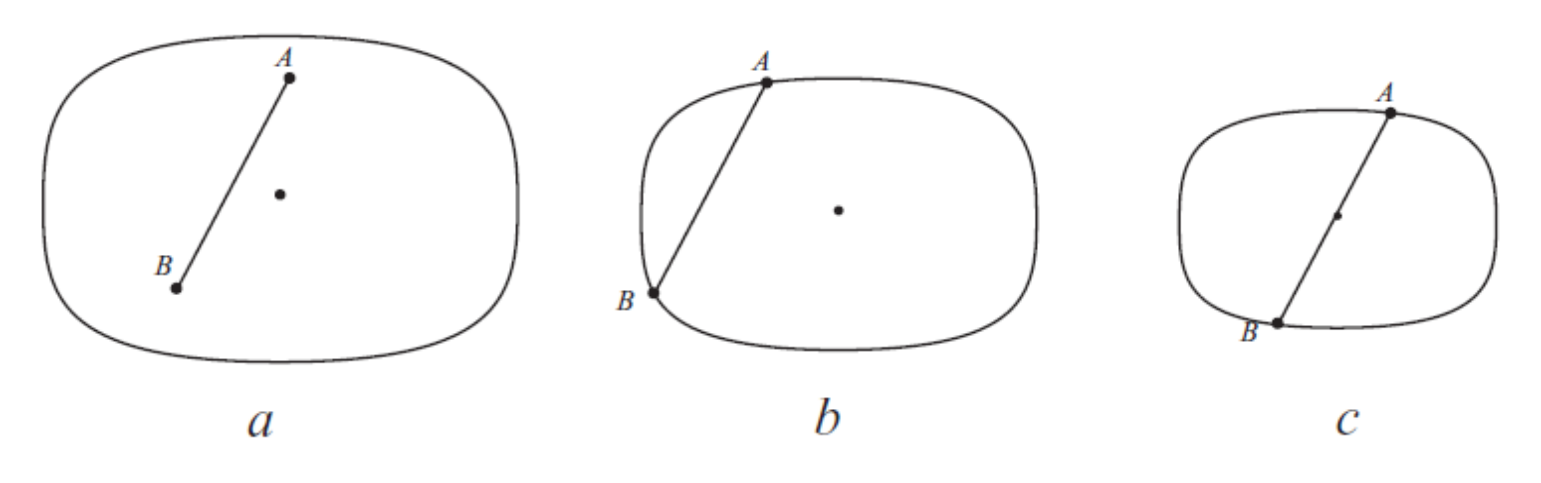
\includegraphics[width=0.9\textwidth]{figures//adaptation.png} 
	\caption{Finding the appropriate state for an affine load path A-B(\cite{koutiri2011effet}).}
	\label{fig.adaptation}
\end{figure}

The effect of the mean stress is taken into account by the term of hydrostatic deformation. The hydrostatic pressure is related to the hydrostatic plastic deformation. 
\begin{equation}
\Sigma_{h,m}=\left( \dfrac{4p_1^2c}{f_cln(f_c)}\left( 1-f_c\right)+3k^{\ast} \right) \epsilon_{h,m}^p.
\label{eq.monchiet9}
\end{equation}
In Eq.\eqref{eq.monchiet9}, $c$ and $k^{\ast}$ are parameters related respectively to the kinematic hardening and to the homogenization scheme.

The parameters of the loading can be linked to the parameters of work-hardening thanks to the relations representative of the adapted state, which are presented in Eq.\eqref{eq.monchiet1}, Eq.\eqref{eq.monchiet9} and Eq.\eqref{eq.monchiet10} to Eq.\eqref{eq.monchiet13}.

The parameter $\xi_{cum}^h$ can not be obtained analytically. On the basis of numerical simulations, the authors propose an approximate expression:
\begin{equation}
\xi_{cum}^h=\dfrac{\sqrt{3}\tau_0}{R_0}\left\lbrace \dfrac{\Sigma_{h,a}}{2\tau_0}-1+exp\left(-\dfrac{\Sigma_{h,a}}{2\tau_0} \right) \right\rbrace .
\label{eq.monchiet17}
\end{equation}





The implementation of this criterion requires the identification of 12 parameters:
\begin{flushleft}
	\qquad - \qquad two parameters, $\gamma_c$ and $\epsilon_c$ linked to the local criterion.\\
	\qquad - \qquad two parameters, $A_0$ and $k_a$, related to the mechanisms of nucleation of cracks.\\
	\qquad - \qquad three parameters related to hardening, $R_0$ And $\tau_0$ linked to the isotropic hardening, $c$ linked to  the kinematic hardening\\
	\qquad - \qquad two coefficients linked to the homogenization scheme, $\mu$ and $k$.\\
	\qquad - \qquad a cubic anisotropy coefficient of the grain $p_1$\\
	\qquad - \qquad a latent coefficient of strain hardening h\\
	\qquad - \qquad a critical porosity coefficient $f_c$\\
\end{flushleft}

\textit{All of these parameters are microscopic, which poses a problem in their identification. Some elements of this modeling have been taken up by \cite{charkaluk2009revisiting}, \cite{charkaluk2007approche} in dissipative approaches. The limitation of this method is that it still requires cycle counting which in complex load case is not feasible.}

\section{Calculation method without cycle counting}
This part presents the existing method of prediction of lifetime, which does not need the algorithm of cycle counting. These kind of methods are still minority and usually more delicate to implement, but present the advantage of free the choice of variable of counting proved to be ``dangerous''. The method presented here is the morel method which is based on stress.

\subsection{Morel's method}
Morel's method (\cite{Morel2000101}) is based on a mesoscopic approach of critical plane type with the
choice of plastic deformation as mesoscopic cumulative damage variable. The description below is taken from his paper. Multiaxial and variable amplitude loading can be analyzed with this method.
To depict the fatigue crack initiation phenomenon in polycrystalline metallic materials, two scales of description of a material will be distinguished: the usual macroscopic scale and a mesoscopic one. The macroscopic scale is defined with the help of an elementary volume
V determined at any point O of a body as the smallest sample of the material surrounding O that can be considered to be homogeneous. V contains a large number of grains (crystals) and the
mesoscopic scale is defined as a small portion of this
volume. In the high cycle fatigue regime, some grains
undergo local plastic strain while the rest of the matrix
behaves elastically (the overall plastic strain is
negligible).

\begin{flushleft}
	Macroscopic quantities. They are:
	\begin{table}[!h]
		\begin{tabular}{lllll}
			$\uline{\uline{\Sigma}}$ & macroscopic stress tensor &  &  &  \\
			$\uline{\uline{E}}$ & macroscopic strain tensor &  &  &  \\
			${\uline{C}}$ & macroscopic shear stress vector  &  &  &  \\
			${\uline{T}}$ & macroscopic resolved shear stress vector acting on an easy glide direction&  &  &  \\
			$T_a$ & amplitude of the macroscopic resolved shear stress  &  &  &  \\	
			$P$ & macroscopic hydrostatic stress.&  &  &  \\	
		\end{tabular}
	\end{table}
	
	Mesoscopic quantities. They are:
	\begin{table}[!h]
		\begin{tabular}{lllll}
			$\uline{\uline{\sigma}}$& mesoscopic stress tensor &  &  &  \\
			$\uline{\uline{\varepsilon}}$ & mesoscopic strain tensor &  &  &  \\
			$\uline{\tau}$& mesoscopic resolved shear stress vector acting on an easy glide direction &  &  &  \\
			$\gamma^p$& mesoscopic shear plastic strain &  &  &  \\
			$\Gamma$ & accumulated plastic mesostrain &  &  &  \\
			$H$ & phase-difference coefficient.&  &  &  \\
		\end{tabular}
	\end{table}
\end{flushleft}

\newpage
\textbf{Constant amplitude loading}
\vspace{6pt}

\textbf{Local stress estimation in high cycle fatigue}

By assuming that only one glide system (defined by a normal vector $\uline{n}$ to a plane and a vector
(direction) $\uline{m}$ within this plane) is active for every plastically deforming grain of the metal, \cite{papadopoulos1993fatigue}
established a macro–meso passage for a glide system activated in a flowing crystal:
\begin{equation}
\uline{\tau}=\uline{T}-\mu\gamma^p\uline{m}
\label{macromeso}
\end{equation}
where $\uline{\tau}$ and $\uline{T}$ are the mesoscopic and macroscopic
resolved shear stresses acting along the slip direction $\uline{m}$ and are defined by:
\begin{equation}
\uline{\tau}=(\uline{m}\cdot\uuline{\sigma}\cdot\uline{n})\uline{m}
\label{tau}
\end{equation}
\begin{equation}
\uline{T}=(\uline{m}\cdot\uuline{\Sigma}\cdot\uline{n})\uline{m}
\label{T}
\end{equation}
and $\gamma^p$  is  the magnitude of the plastic mesoscopic shear strain deduced from the plastic flow rule associated to Eq.\eqref{Schmid}.
\begin{figure}[h!]
	\centering
	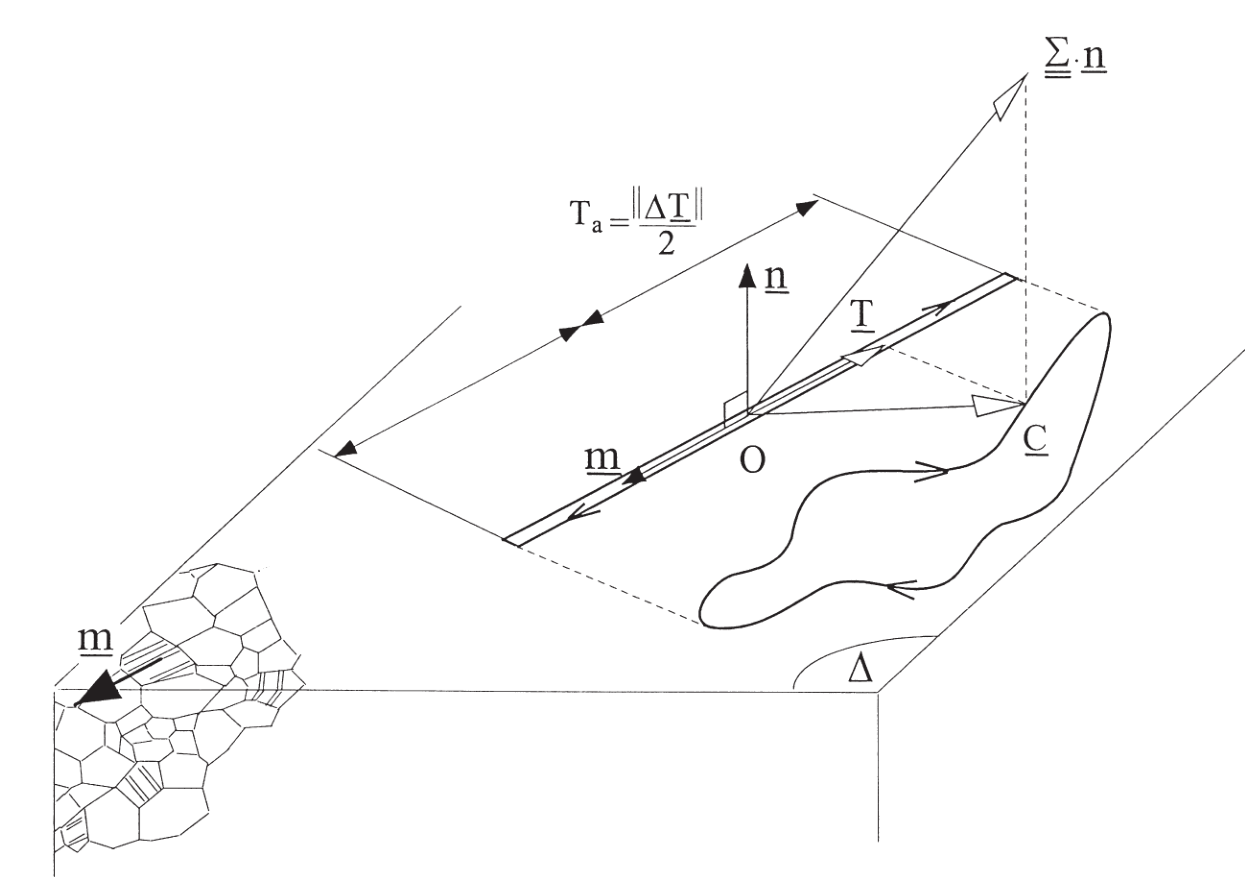
\includegraphics[width=0.8\textwidth]{figures//glid.png} 
	\caption{Path of the macroscopic shear stress $\uline{C}$ acting on a material plane $\Delta$ and the corresponding path of the macroscopic resolved shear stress $\uline{T}$ acting on an easy glide direction (\cite{Morel2000101}).}
	\label{glid}
\end{figure}


Schmid's law with isotropic and kinematic hardening:
\begin{equation}
f(\uline{\tau},\uline{b},\tau_y)=(\uline{\tau}-\uline{b})\cdot(\uline{\tau}-\uline{b})-\tau_y^2=0
\label{Schmid}
\end{equation}
where $\uline{b}$ is the kinematic back stress, and $\tau_y$ is the yield limit subjected to hardening.

Three successive linear isotropic hardening rules have
been adopted on $\tau_y$ to describe the crystal behavior from
initial yield to failure (\figref{3phases}a). The damage variable is the accumulated plastic mesostrain $\Gamma$ (\figref{3phases}b).
In the first phase, we have a linear increase $\dot{\tau}_y=g\dot{\Gamma}$, in the second phase when $\tau_y$ reaches a saturation $\tau_{lim}$, $\dot{\tau}_y=0$, and then above a certain threshold, we have softening $\dot{\tau}_y=-h\dot{\Gamma}$.

In the description and implementation of his method, Morel draws heavily on the work developed by Papadopoulos including the use of a measure of cumulative mesoscopic plastic deformation   and modeling the behavior of grain in three distinct phases (hardening, saturation and softening); he considers the cumulative mesoscopic plastic deformation $\Gamma$ as damage parameter and assumes that the initiation of a fatigue crack occurs when the latter reaches a
critical value $D = D_R = \Gamma_R$ (\figref{3phases}). 
\begin{figure}[h!]
	\centering
	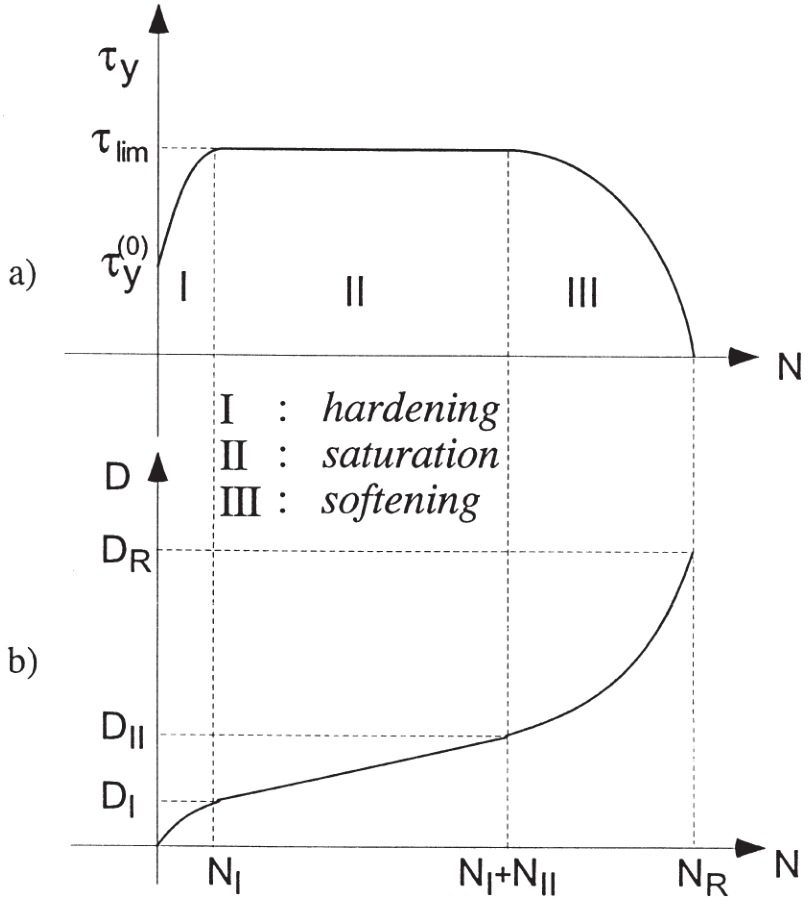
\includegraphics[width=0.5\textwidth]{figures//3phases.png} 
	\caption{(a) Yield limit evolutions and (b) damage evolution in the three behavior phases (hardening, saturation and softening) when a cyclic loading is applied (\cite{Morel2000101}).}
	\label{3phases}
\end{figure}

\begin{figure}[h!]
	\centering
	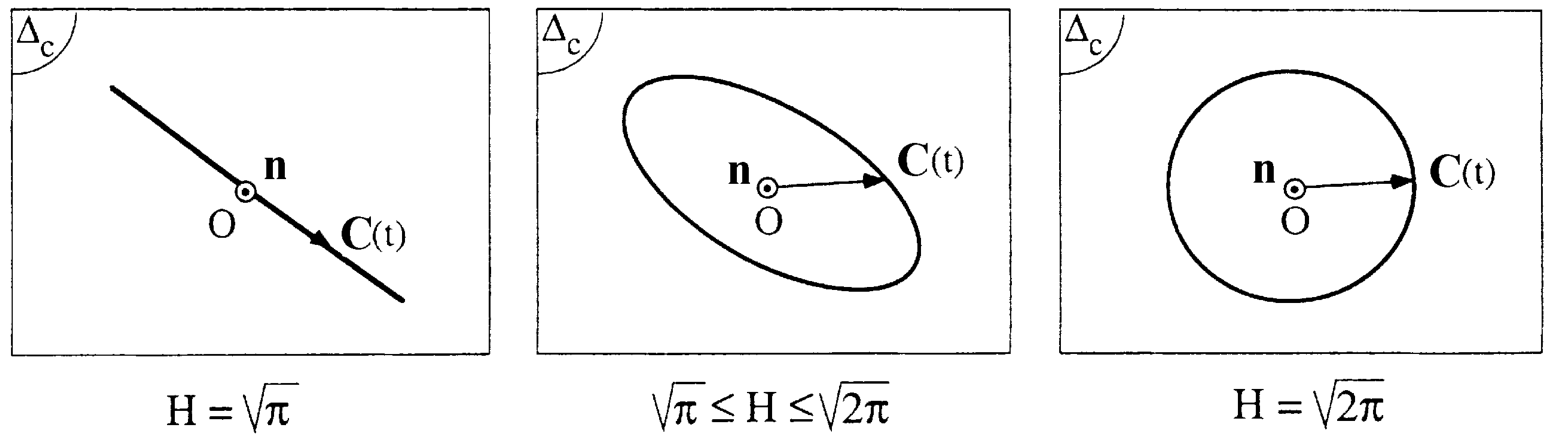
\includegraphics[width=0.9\textwidth]{figures//H.png} 
	\caption{Different paths of loading in the plane and corresponding values of the phase-difference coefficient $H$ (\cite{Morel2000101}). For a proportional loading, H is equal to $\sqrt{\pi}$. In the case of a particular
		circular path, H reaches the maximum value $\sqrt{2\pi}$ (\figref{figH}). 
		The linear path and the circular one lead to two bounds of
		the coefficient H.}
	\label{figH}
\end{figure}

\vspace{6pt}
\textbf{Number of cycles to failure}
\vspace{6pt}

Once the accumulated plastic mesostrain $\Gamma$ along the particular gliding system reaches a critical value $\Gamma_R$, these grains are said to be broken. An analytical expression of the number
of cycles to initiation (S–N curve) can be achieved:
\begin{equation}
\Gamma=\Gamma_R \, \Rightarrow \, N_i=pln\left(\frac{C_A}{C_A-\tau_{lim}}\right)+q\left(\frac{\tau_{lim}}{C_A-\tau_{lim}}\right)-\frac{r}{C_A}
\label{eq.morelNF}
\end{equation}
where $p$, $q$ and $r$ are functions of the hardening parameters of the three phases defined above.

From Eq.\eqref{taus} we can find the yield point $\tau_s$ of the crystal in the saturation phase as a function of the amplitude $P_a$ and the mean value $P_m$ of the hydrostatic pressure, the phase difference of coefficient $H$ and two material related parameters $\alpha$ and $\beta$ :
\begin{equation}
\tau_{lim}=\tau_s=\frac{-\alpha P_m+\beta}{\alpha\frac{P_a}{C_A}+H}
\label{taus}
\end{equation}
In the last relation Eq.\eqref{eq.morelNF}, the detrimental effect of out-
of-phase loading is introduced through $\tau_{lim}$. As the coefficient H increases, $\tau_{lim}$ as well as $N_i$ decrease and therefore more damage is accumulated. The identification of
the model parameters requires two endurance limits
(parameters a and b of the endurance criterion) and a
single S–N curve (parameters $p$, $q$ and $r$).

The fatigue control mechanism is embedded in the construction of the saturation limit $\tau_{lim}$ of $\tau_y$ which is constructed separately on each slip system using fatigue test data. More precisely, we assume that the given material has an endurance limit in uniaxial loading given as in Papadopoulos by
$$\Delta T/2+\alpha P_{max}=\beta$$
with material coefficients $\alpha$ and $\beta$, $\Delta T/2$ the amplitude of the resolved shear stress, and $P_{max}$ the maximum hydrostatic stress. For a given cyclic shear loading on the considered slip line of amplitude $T_a$, average hydrostatic stress $P_m$ and amplitude of hydrostatic stress $P_a$, we introduce the amplitude scaling $k$ where we have
$$kT_a+\alpha\left( kP_a+P_m\right)=\beta  $$
which is given by
 $$ k=\dfrac{\beta-\alpha P_m}{T_a+\alpha P_a}$$ 
 and which will send this loading to the endurance curve, and a shape factor $\sqrt{\pi}\leqslant H\leqslant \sqrt{2\pi}$ characterizing the shape of the loading path in the considered plane of normal $\uline{n}$ (Figure.\ref{figH}). The local saturation limit $\tau_{lim}(\uline{m},\uline{n})$ is then defined by the amplitude of the shear loading $T_a$ once multiplied by the scaling factor $k$ and corrected by the shape factor $H$, giving
$$\tau_{lim}(\uline{m},\uline{n})=\frac{k}{H}T_a(\uline{m},\uline{n})=\frac{1}{H}\frac{\beta-\alpha P_m}{T_a+\alpha P_a}T_a(\uline{m},\uline{n}).$$

\vspace{6pt}
\textbf{General loading}
\vspace{6pt}

 In this framework, Morel's method uses three successive steps for computing the damage created by repeated loading sequences:

\begin{enumerate}
\item Find the critical plane $\uline{n}$ maximizing the in-plane plastic deformation $\int_{\uline{m}}\gamma^p$ which will be induced by the loading sequence, assuming linear isotropic hardening without saturation.
\item On this plane  $\uline{n}_c$, on each direction $\uline{m}$, compute the plastic history, that is
\begin{enumerate}
	\item compute the shear history $T(t)=\uline{m}\cdot \uline{\uline{\Sigma}}\cdot \uline{n}_c$
	\item decompose in local loading cycles $(i)$ counted $n_{(i)}$ times with load amplitude $T_a^{(i)}$, mean hydrostatic load of mean $P_m^{(i)}$ and amplitude $P_a^{(i)}$, using a standard scalar rainflow counting method (chapter \ref{chp:4})
	\item compute the local saturation limit $$\tau_{lim}^{(i)}=\frac{1}{H}\frac{\beta-\alpha P_m^{(i)}}{T_a^{(i)}+\alpha P_a^{(i)}}T_a^{(i)}$$ and its sequence average $\left\langle \tau_{lim} \right\rangle$ 
	\item compute the accumulated plastic strain 
	\begin{equation}
\Gamma_{\uline{m},\uline{n}_s}=\sum_{(i)}n_{(i)}\dfrac{4}{c+\mu}\left(T_a^{(i)}-\tau_{lim}^{(i)} \right)_+
\label{eq.morel_plastic}
	\end{equation}
\end{enumerate}
\item Find the critical direction $\uline{m}_s$ maximizing among the directions $\uline{m}$ with the accumulated plastic strain $\Gamma_{\uline{m_s},\uline{n}_s}$, and use this accumulated plastic strain to compute the incremental damage occurring during the repeated loading sequence
\begin{equation}\Delta D=l\dfrac{\Gamma_{\uline{m_s},\uline{n}_s}}{\left\langle \tau_{lim} \right\rangle_{\uline{m_s},\uline{n}_s}}
	\label{NFsimple}
\end{equation}
thus assuming linear damage accumulation.
\end{enumerate}

With the present way, a new counting method is defined. Indeed, damage is deduced step by step from
the hardening rules. Each time the plasticity criterion is
violated (the yielding sphere is exceeded) some plastic
strain is accumulated and then damage increases. This
fact is quite new because most of the fatigue life prediction methods in the literature successively apply a counting method (e.g. ``Rainflow method'') and a damage law
(e.g. Miner rule), without any link between them. The
choice of accumulated plastic mesostrain as damage
variable and the use of appropriate hardening rules seem
then to be a promising and efficient way to understand
and describe the physical mechanisms of crack
nucleation.

\vspace{6pt}
\textbf{Experimental verification}
\vspace{6pt}

\textbf{In case of constant amplitude test }
\vspace{6pt}

The author \cite{FFE:FFE452} consider the example of an out-of-phase bending-torsion test on a high strength steel (30NCD16). The endurance limits of this material in reversed
bending and torsion are, respectively, $f=680\,\textnormal{MPa}$ and $t=426\,\textnormal{MPa}$.  The multiaxial sinusoidal loading is characterized by the amplitudes $\Sigma_{11a} =600\,\textnormal{MPa}$, $\Sigma_{12a} =335\,\textnormal{MPa}$ (no mean stresses)
and the phase difference $\beta_{12} =90°$.

The maximum value of $T_\sigma$ (denoted as $T_\Sigma$ ) can be deduced numerically. For this loading, we find $T_\Sigma=697\,\textnormal{MPa}$. On the critical material
plane (where $T_\Sigma$ is reached), $C_A$ is estimated to be $282\,\textnormal{MPa}$. The phase difference coefficient $H$ is
then simply deduced: $H=T_\Sigma /C_A =2.47$.

Besides noting that $P_m =0\,\textnormal{MPa}$, $P_a=200\,\textnormal{MPa}$ and $a=0.67$, $b=775\,\textnormal{MPa}$, $T_{\Sigma lim}$ is readily
computed with the help Eq.\eqref{taus}: $T_{\Sigma lim} =633\,\textnormal{MPa}$. Finally, $\tau_{lim} =T_{\Sigma lim} /H=256\,\textnormal{MPa}$. Once $p$, $q$ and $r$ have been identified from a $S–N$ curve with the least squares line method, $C_A $and $\tau_{lim}$ can
be introduced into Eq. \eqref{eq.morel_plastic} and the number of cycles to initiation can be finally calculated, i.e.
$N_F =2\times10^5$ cycles.

\vspace{6pt}
\textbf{In case of variable amplitude test }
\vspace{6pt}

According to the previous endurance data and the
definition of the generalized fatigue limit (for bending
$\tau_{lim} =f/2$ and for torsion $\tau_{lim}=t$), one can estimate the parameter $q=20 800$.

\begin{figure}[h!]
	\centering
	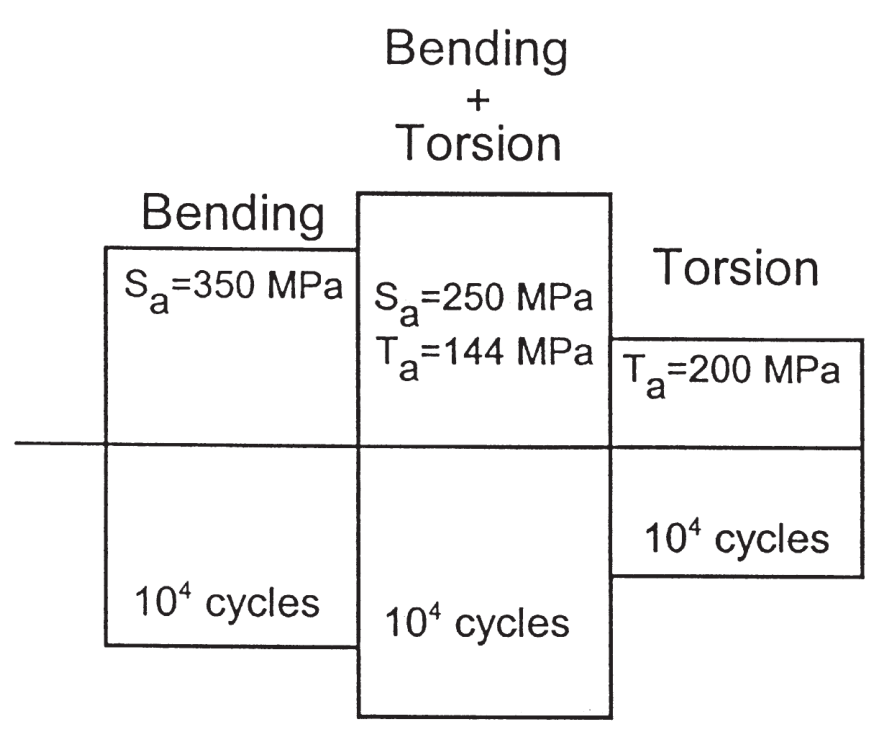
\includegraphics[width=0.6\textwidth]{figures//block.png} 
	\caption{block sequence tests (bending/bending+torsion/torsion) performed on a mild
		steel XC18.}
	\label{block}
\end{figure} 

Let us consider now a block sequence composed of
$10^4$ cycles of bending ($\Sigma_a =350\,\textnormal{MPa}$) followed by $10^4$
cycles of combined in-phase bending-torsion ($\Sigma_a ,T_a =250 \,\textnormal{MPa}, 144 \,\textnormal{MPa}$)
followed by $10^4$ cycles of torsion ($T_a =200\,\textnormal{MPa}$). This
sequence is repeated until the initiation of a crack. The
mean lifetime is found to be $N=1.73\times10^5$ .

The three generalized fatigue
limits relative to the three blocks are estimated according
to Eq.\eqref{taus}:

$$\tau_{lim}^{bending}=155 \,\textnormal{MPa}$$    
$$\tau_{lim}^{torsion}=179 \,\textnormal{MPa}$$  
$$\tau_{lim}^{bend+tors}=157 \,\textnormal{MPa}$$


These three values and the parameter $q$ are enough to
accumulate the damage in the three blocks using Eq.\eqref{NFsimple}:


$$\frac{\Gamma^{(bending)}}{\Gamma_R^{(bending)}}+\frac{\Gamma^{(bend+tors)}}{\Gamma_R^{(bend+tors)}}+\frac{\Gamma^{(torsion)}}{\Gamma_R^{(torsion)}}=1$$

The corresponding number of cycles to initiation is:
$N_{prediction} <1.5\times10^5$ , that is to say five successive applications of the sequence. This prediction, close to the experimental result $N=1.73\times10^5$ , is a conservative one.

It is important to note that if only one critical plane
(either from bending, torsion or bending+torsion
loading) is used for damage accumulation, one-third of
the damage would be calculated, resulting in a nonconservative prediction.

Morel's method is promising in its description aspect of limited endurance fatigue phenomenon, through the choice of the  mesoscopic plastic deformation. By using cumulative plasticity, a fatigue mechanisms occurring at the mesoscopic scale takes into account the main factors affecting the lifetime cycle fatigue (hydrostatic pressure and influence of phase shift). 

However, at the present stage, it does not completely meet the demand of a predictive tool. Indeed, it is a relatively complicated method (search critical plane $\Delta_c$ and accumulated damage in each direction in the plan); its application for multiaxial variable amplitude fatigue loads requires data that are still not available (an S-N curve, two endurance limits and a particular  damage accumulation test). Moreover, it is not completely free of counting method because its author uses the counting of the extrema of the evolution of the resolved shear $T_a$ to get the macroscopic resolved shear stress $T_A$ and the corresponding amplitude $P_a$ and mean values $P_m$ of the hydrostatic stress in each direction (m) in $\Delta_c$. Again, this makes it difficult and daunting task.
